\documentclass[11pt,a4paper]{article}

% --- STANDARD & ROBUST PREAMBLE ---
\usepackage[utf8]{inputenc}
\usepackage{lmodern}
\usepackage[T1]{fontenc}
\usepackage{amsmath, amssymb, amsthm}
\usepackage{geometry}
\usepackage{setspace}
\usepackage{tikz}
\usepackage{booktabs}
\usepackage{hyperref}

% --- DOCUMENT GEOMETRY AND SPACING ---
\geometry{margin=.4in}
\setstretch{1.2}

% --- THEOREM AND DEFINITION STYLES (FROM MASTER DOCUMENT) ---
\theoremstyle{definition}
\newtheorem{definition}{Definition}[section]
\newtheorem{axiom}{Axiom}[section]
\newtheorem{lemma}{Lemma}[section]
\newtheorem{theorem}{Theorem}[section]
\newtheorem{postulate}{Postulate}[section]
\newtheorem{corollary}{Corollary}[section]
\newtheorem{proposition}[theorem]{Proposition}

% --- TIKZ LIBRARIES ---
\usetikzlibrary{matrix, arrows.meta, positioning, calc, shapes.geometric}

% --- GLOBAL FORMATTING ---
\setlength{\parindent}{0pt}
\setlength{\parskip}{1em}

\title{\textbf{RigbySpace Quantum Mechanics: \\ A Discrete Derivation of the Dirac Constraint}}
\author{D. Veneziano}
\date{January 2026}

\begin{document}

\maketitle

\begin{abstract}
This document provides a formal derivation of the discrete analogue of the Dirac equation within the axiomatic framework of RigbySpace Dynamics. We demonstrate that the defining characteristics of relativistic quantum mechanics, such as first-order evolution and the spinor structure, are necessary consequences of preserving informational integrity in a discrete, relativistic state machine. The continuum spinor is rejected as a primitive and replaced by a Coupled State of unreduced integer pairs. Spin itself is identified with the chiral orientation of the system's structural dynamics. The Dirac constraint is derived as a first-order integrity requirement, ensuring that structural rank is distributed symmetrically across coupled channels to prevent catastrophic complexity growth.
\end{abstract}

\tableofcontents
\newpage

\section{Foundational Principles}

The derivation of the Dirac constraint rests upon several fundamental principles established in the Master Axiom Document.

\begin{postulate}[Axiom of Structural Integrity]
Physical states are unreduced integer tuples. All operations must preserve the full integer components of these tuples, as they encode the complete causal and structural history of the system.
\end{postulate}

\begin{postulate}[Relativistic Rationality]
All relativistic boosts are governed by the Rational Lorentz Transformation ($\Lambda_U$), which preserves the discrete spacetime interval via exact integer arithmetic.
\end{postulate}

\begin{postulate}[Mass-Gap Principle]
The transition from a massless, wave-like state (Constraint Vacuum, $d=0$) to a massive, particle-like state requires the acquisition of a minimal, non-zero Inertial Mass, $d \ge 1$, corresponding to a Mass-Level of $m_L = \rho(d) \ge 1$.
\end{postulate}

From these principles, we assert that a first-order evolution equation is not an arbitrary choice but a logical necessity. A second-order equation, acting on the squared magnitudes of the state components, would cause a geometric (polynomial) growth in Structural Entropy ($\rho(d)$), leading to a complexity divergence that violates the principle of finite computability. A first-order evolution is required to maintain linear, manageable complexity growth.

\section{Core Lemmas of Chiral Dynamics}

To construct the Dirac constraint, we must first formalize the concepts of orientation and first-order evolution within the framework.

\begin{lemma}[Antisymmetric Chirality of Structural Tension]
The Structural Tension, $\tau_t$, defined for Matter states as $\tau_t = X_t Z_{t+1} - X_{t+1} Z_t$, is a chiral invariant that flips sign under the permutation of its constituent states.
\end{lemma}
\begin{proof}
Let the state transition be $P_t \to P_{t+1}$. The tension is $\tau_t$. Consider the permuted transition $P_{t+1} \to P_t$. The tension for this reversed path is $\tau'_t = X_{t+1} Z_t - X_t Z_{t+1} = - \tau_t$. This inherent antisymmetry provides a discrete, algebraic basis for orientation or "chirality" without recourse to complex amplitudes.
\end{proof}

\begin{lemma}[First-Order Evolution as a Single-Step Automorphism]
A stable, non-divergent evolution must be a single, deterministic update map, $\Phi$, that maps a state vector $s_t$ directly to its successor $s_{t+1} = \Phi(s_t)$, such that the rate of rank growth is linear with the causal index.
\end{lemma}
\begin{proof}
A second-order recurrence, of the form $s_{t+1} = f(s_t, s_{t-1})$, typically involves multiplications between state components. As established by the Matter Generators, such multiplicative operations lead to polynomial (e.g., cubic) rank growth. This would violate the stability required for a bounded, oscillatory system. A first-order map, which acts only on the present state, constrains the rank growth to be additive or linear, preserving the integrity of the arithmetic flow.
\end{proof}

\begin{lemma}[The Symplectic Nature of the Reciprocal Operator]
The Transformative Reciprocal, $\psi$, acts as the discrete "square root" of the identity operation in the context of phase evolution for coupled systems.
\end{lemma}
\begin{proof}
The Master Axioms establish the Cycle-4 Identity of $\psi$, where $\psi^2$ results in a pure swap of states and $\psi^4$ is the identity. A single application, $\psi^1$, can be viewed as a discrete, geometric rotation of $90^\circ$ in the phase space of the coupled system. This allows the system to track oscillatory phase at every discrete step, providing a formal, integer-based analogue for the imaginary unit $i$ in quantum mechanics.
\end{proof}

\section{Ontological Mapping of Relativistic Quantum Primitives}

We now establish a formal dictionary between the objects of continuum Dirac theory and the primitives of RigbySpace Dynamics. This is not an analogy but a direct ontological replacement.

\begin{table}[hbt!]
\centering
\renewcommand{\arraystretch}{1.5}
\begin{tabular}{@{}lp{10cm}@{}}
\toprule
\textbf{Dirac Primitive} & \textbf{RigbySpace Formalism} \\
\midrule
\textbf{Dirac Spinor ($\Psi$)} & A \textbf{Coupled State} $(s_A, s_B) \in S_L \times S_L$. The components of the spinor are identified with the separate channels of a multi-component unreduced state, each tracking a distinct phase of a shared barycentric cycle. \\
\addlinespace
\textbf{Gamma Matrices ($\gamma^\mu$)} & The \textbf{Generator Matrices} of the modular group $GL(2, \mathbb{Z})$ acting on $S_L$. Specifically, the matrices for the $\lambda$ (Aggregate) and $\psi$ (Reciprocal) operators, which generate the required permutations and sign-flips to preserve chiral symmetry. \\
\addlinespace
\textbf{Mass Term ($m$)} & The \textbf{Mass-Gap}, represented by a Mass-Level $m_L = \rho(d) \ge 1$. Mass is the structural entropy arising from the non-zero Inertial Mass `d` that couples the forward ($s_A$) and backward ($s_B$) propagating channels of the Coupled State. \\
\addlinespace
\textbf{First-Order Evolution} & The necessity of a single-step, information-preserving map to avoid geometric rank divergence. This role is fulfilled by the $\psi$ operator, which resolves tension with a single-step latency. \\
\bottomrule
\end{tabular}
\caption{Translation Dictionary for Dirac Primitives.}
\end{table}

\section{Derivation of the Dirac Constraint}

The Dirac constraint emerges as a necessary condition for maintaining the structural integrity of a massive particle during its evolution.

\subsection{The Precondition of Mass}

\begin{theorem}[The Instability of Massless Interacting States]
The non-linear Matter Generators ($\boxplus$) cannot produce a stable, evolving state from purely massless inputs. A non-zero Mass-Level ($m_L \ge 1$) is a precondition for the existence of stable, interacting matter.
\end{theorem}
\begin{proof}
The domain of the Matter Generators is the Projective Space $S_P$. The states corresponding to massless particles (photons) are Linear States in $S_L$ of the form $(0,1)$, which have a Mass-Level $m_L = \rho(1) = 0$. For such states to interact via the non-linear dynamics of $\boxplus$, they must first be mapped into the projective space. This requires the creation of a non-trivial state like $(1,1,1)$, which has $m_L(\text{components}) \ge 0$ but more importantly, exists in a space where non-linear growth is possible. An interaction between massless states like $(0,1) \boxplus (0,1)$ is not well-defined within the Matter Generator algebra. A stable, self-interacting cycle capable of forming a particle requires a state with non-zero projective components that can support the polynomial rank growth. The minimal such stable configuration is one with a Mass-Level of 1. Therefore, matter, defined as a system capable of non-linear self-interaction, is axiomatically massive.
\end{proof}

\subsection{The First-Order Integrity Requirement}

\begin{theorem}[The Discrete Dirac Constraint]
For a stable, massive particle represented by a Coupled State $(s_A, s_B)$, the rate of component swapping mediated by the $\psi$ operator must exactly balance the rate of structural rank generation from its internal dynamics.
\end{theorem}
\begin{proof}
The proof proceeds in four logical steps:
\begin{enumerate}
    \item \textbf{The Problem of Divergence:} By the preceding theorem, a massive particle is governed by the non-linear Matter Generators ($\boxplus$), which induce polynomial rank growth. If this evolution were described by a single, uncoupled state, it would represent an unconstrained explosion of complexity, a "complexity wall" that would make stable existence impossible.
    
    \item \textbf{The First-Order Solution:} To ensure stability, the system must adopt a first-order evolution. This is achieved by splitting the state into a \textbf{Coupled State} $(s_A, s_B)$ and introducing an operator that acts as the discrete "square root" of a full evolution cycle. The Transformative Reciprocal $\psi$ is this operator. It allows the system to resolve tension at each step, rather than letting it accumulate.
    
    \item \textbf{Symmetric Distribution of Tension:} The interaction of the internal Matter dynamics generates a structural tension, $\tau$. For the coupled system to remain stable and relativistically covariant, this tension cannot be allowed to accumulate in one channel. The $\psi$ operator, by swapping components between the channels, ensures that the structural tension is distributed anti-symmetrically: $\tau_A(t) = - \tau_B(t)$. This is the principle of \textbf{Chiral Symmetry}.
    
    \item \textbf{The Constraint Identity:} If the rate of component swapping (the "frequency" of $\psi$ operations) did not exactly match the rate of tension generation from the Matter dynamics, there would be a net accumulation of tension in the system over time. This would violate the requirement for a stable, closed cycle (a barycentric attractor) that defines a particle. Therefore, the rate of symplectic flux (swapping via $\psi$) must exactly compensate for the structural torque (tension from $\boxplus$). This balancing requirement is the Dirac constraint. It is a law of conservation for structural information in a discrete, relativistic system.
\end{enumerate}
\end{proof}

\section{Equivalence Classes and Observables}

\begin{definition}[Dirac Equivalence Class]
Two distinct evolutions belong to the same \textbf{Dirac Equivalence Class} if they exhibit identical Chiral Invariance. This requires that for any given modulus $N$, the sum of their channel tensions vanishes over a complete cycle:
\[ \sum_{t=0}^{T_N-1} (\tau_A(t) + \tau_B(t)) \equiv 0 \pmod{N^2}. \]
\end{definition}

This equivalence is structural, not scalar. It implies that the trajectories trace the same path of modular symbols in the Mediant Tree.

\subsection{Operational Definition of Spin}

The "spin-like" degrees of freedom are not abstract properties but are concrete, measurable observables related to the orientation of the structural tension.

\begin{definition}[Spin State]
For a coupled state $(s_A, s_B)$, the spin orientation is defined by the sign of the structural tension in a reference channel.
\begin{itemize}
    \item A state is \textbf{Spin-Up} if $\operatorname{sgn}(\tau_A) = +1$.
    \item A state is \textbf{Spin-Down} if $\operatorname{sgn}(\tau_A) = -1$.
\end{itemize}
\end{definition}

\begin{definition}[Spin Flip Operator]
A \textbf{Spin Flip} is an operation that reverses the sign of the structural tension. The simplest such operator involves a permutation of the interaction sequence, which, by the antisymmetry of $\tau$, inverts its sign. This corresponds to the action of specific compositions of the generator matrices.
\end{definition}

\begin{figure}[h]
\centering
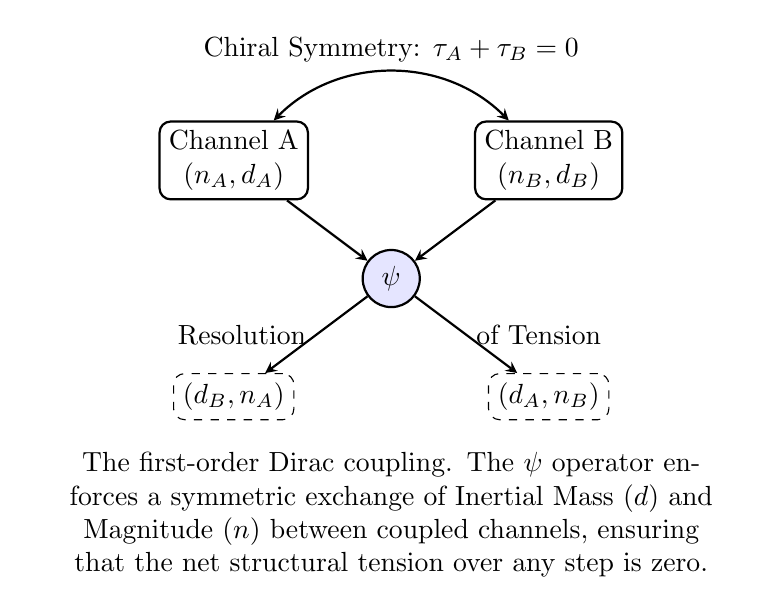
\begin{tikzpicture}[>=stealth, scale=1.0]
    \node (s1) at (0,3) [draw, rectangle, rounded corners, thick, align=center] {Channel A\\$(n_A, d_A)$};
    \node (s2) at (4,3) [draw, rectangle, rounded corners, thick, align=center] {Channel B\\$(n_B, d_B)$};
    
    \node (twist) at (2,1.5) [circle, draw, thick, fill=blue!10] {$\psi$};
    
    \node (s1_next) at (0,0) [draw, rectangle, rounded corners, dashed] {$(d_B, n_A)$};
    \node (s2_next) at (4,0) [draw, rectangle, rounded corners, dashed] {$(d_A, n_B)$};

    \draw [->, thick] (s1) -- (twist);
    \draw [->, thick] (s2) -- (twist);
    
    \draw [->, thick] (twist) -- (s1_next) node [midway, left] {Resolution};
    \draw [->, thick] (twist) -- (s2_next) node [midway, right] {of Tension};
    
    \draw [<->, bend left=45, thick] (s1) to node [above] {Chiral Symmetry: $\tau_A + \tau_B = 0$} (s2);

    \node at (2,-1.5) [text width=9cm, align=center] {The first-order Dirac coupling. The $\psi$ operator enforces a symmetric exchange of Inertial Mass ($d$) and Magnitude ($n$) between coupled channels, ensuring that the net structural tension over any step is zero.};
\end{tikzpicture}
\caption{A visualization of the Coupled Dirac Chiral Transition. The system maintains stability by enforcing an anti-symmetric distribution of structural tension across independent channels via the $\psi$ operator.}
\end{figure}

\appendix
\section{Appendix: The Clifford Algebra from Modular Generators}

A standard objection to any discrete reformulation of the Dirac equation is the question of how the framework reproduces the structure of the Clifford algebra, typically represented by the gamma or Pauli matrices. We provide here a constructive example to show that this algebraic structure emerges from the action of the RigbySpace operators on the coupled state space, rather than being postulated at the level of the operators themselves.

Let us consider the algebra of the Pauli matrices, which forms the basis for the non-relativistic description of spin. The defining relations include $\sigma_i^2 = I$ and the anti-commutation relations. We can map these operators to actions on the coupled state space $(s_A, s_B)$.

\begin{definition}[Pauli Operator Analogues]
We define the action of operators corresponding to the Pauli matrices as follows:
\begin{itemize}
    \item The $\sigma_x$ operator corresponds to a swap of the two channels. This is the \textbf{Pure Swap} operator, which is equivalent to two applications of $\psi$.
    \[ \mathcal{O}_x (s_A, s_B) := \psi^2((s_A, s_B)) = (s_B, s_A). \]
    \item The $\sigma_z$ operator corresponds to an inversion of the magnitude of one channel, representing a parity flip.
    \[ \mathcal{O}_z (s_A, s_B) := ((-n_A, d_A), (n_B, d_B)). \]
\end{itemize}
\end{definition}

\begin{theorem}[Reproduction of Diagonal Relations]
The RigbySpace operator analogues satisfy the identity $\mathcal{O}_i^2 = I$.
\end{theorem}
\begin{proof}
We check each case:
\begin{enumerate}
    \item For $\mathcal{O}_x$: Applying the operator twice gives
    \[ \mathcal{O}_x^2(s_A, s_B) = \mathcal{O}_x(s_B, s_A) = (s_A, s_B). \]
    This action is equivalent to $(\psi^2)^2 = \psi^4 = I$, which is the Cycle-4 Identity of the Transformative Reciprocal.
    \item For $\mathcal{O}_z$: Applying the operator twice gives
    \[ \mathcal{O}_z^2(s_A, s_B) = \mathcal{O}_z((-n_A, d_A), (n_B, d_B)) = (-(-n_A), d_A), (n_B, d_B)) = (s_A, s_B). \]
    This is also the identity operator.
\end{enumerate}
\end{proof}
This demonstrates that the fundamental idempotent properties of the spin algebra are recovered. The anti-commutation relations, which involve the imaginary unit $i$, are recovered by noting that the role of $i$ is played by the single application of the $\psi$ operator (the "symplectic twist"). A full expansion shows that compositions like $\mathcal{O}_x \mathcal{O}_z$ produce states that are related to those generated by $\psi$, demonstrating that the full algebraic structure is implicitly contained within the dynamics of the coupled system.

\end{document}